\chapter{Results} \label{ch:results}

%----------------------------------------
% EXPERIMENTS
%----------------------------------------
\section{Experiments}

	The experiments were run using Cessna 172S flight data produced by students at the University of North Dakota during the month of September 2015.  Student flight data is ideal for unstable analysis testing as it contains very noisy data, which provides a diverse array of flying patterns.  A random sample of 100 flights was chosen for the experiments.
        
    First, the application was run against the 100 flights to obtain the automated analysis results.  The same 100 flights were then manually analyzed in order to get human results for the phase identification, which could be compared to the automated results then determine the accuracy of the application.  The test of the 100 flights was also run ten times each with the single-process version and the multi-process version as previously described.  This was done in order to compare and contrast the performance of the separate versions.


%----------------------------------------
% ACCURACY OF PHASE IDENTIFICATION
%----------------------------------------
\section{Accuracy of Phase Identification}

	The manual validation was performed using a combination of tools available on the NGAFID website:  the Cesium flight reanimation tool and the Keyhole Markup Language (KML) generator to visualize the flight path in \textit{Google Earth}~\cite{nolan2014keyhole} (see \Cref{fig:kml_example}).
    
    \begin{figure}
    	\centering
        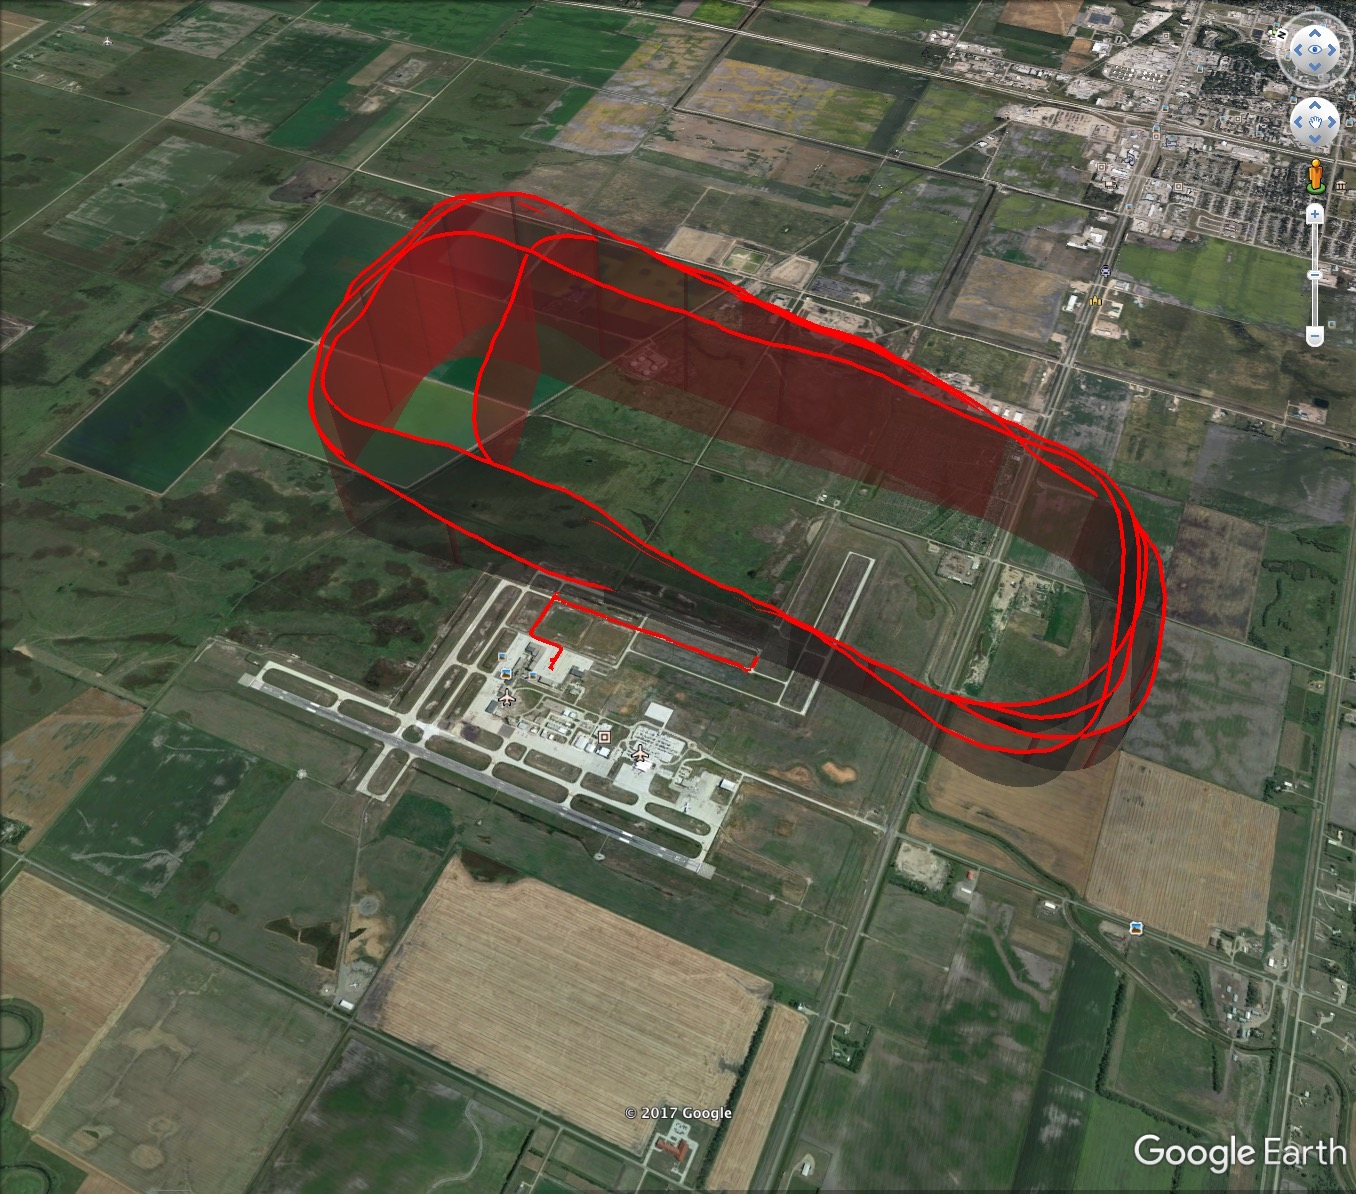
\includegraphics[width=\linewidth]{img/kml_example}
        \caption{Example of using a KML file to visualize a flight path in \textit{Google Earth}.  This flight visualization is an example of a student flight that has multiple Approach phases.}
        \label{fig:kml_example}
    \end{figure}
    
    
    %----------
    % APPROACH
    %----------
    \subsection{Approach}
    
        The \toolname\ generated a total of 377 approaches for the 100 flights that were tested. As seen in \Cref{fig:kml_example}, student flights typically consist of multiple approaches as this is something that needs to be practiced.  Out of the total; there are 370 (98.14\%) true positives, five (1.33\%) false positives, and two (0.53\%) false negatives.  These results can also be found in \Cref{fig:validation_results}.  In the context of this application, a true positive is a case where the tool correctly indicates that an approach is occurring during a specified time frame.  A false positive occurs when the tool indicates that an approach is occurring but is not in reality.  Typically, a false positive occurs when the flight data has invalid values for about the first ten rows, which then throws off the beginning of the algorithms.  This happens infrequently, but could be accounted for in a future work by sanitizing the data before analysis.  A false negative is the exact opposite where the tool indicates that an approach is not occurring but it is in reality.  Typically, a false negative occurs when the approached airport's geological data is not contained within the database.  These types of occurrences should stop once the airports database is expanded with more entries.  Lastly, the tool misclassified the approached runway 13 times (3.45\%).  A runway is misclassified when the difference between the aircraft and runway headings is greater than $20^\circ$.  This occurs during the runway detection portion of the approach analysis algorithm, and the algorithm either returns a \emph{null} runway or an incorrect runway due to the large heading difference.

        In this same context, it is difficult to quantify the number of true negatives since these would be cases where the tool correctly indicates that an approach is not occurring.  The difficulty lies in how to define a single occurrence.  Should a single true negative be counted for every second the tool indicates that an approach is not occurring?  If so, then this would create a numerous amount of true negatives and would dilute the percentages of the other statistics, which are more important in this application.

        The validation results demonstrate that the \toolname\ is exceptionally accurate in its ability to appropriately detect and classify most approaches in a flight.

        \begin{figure}
            \centering
            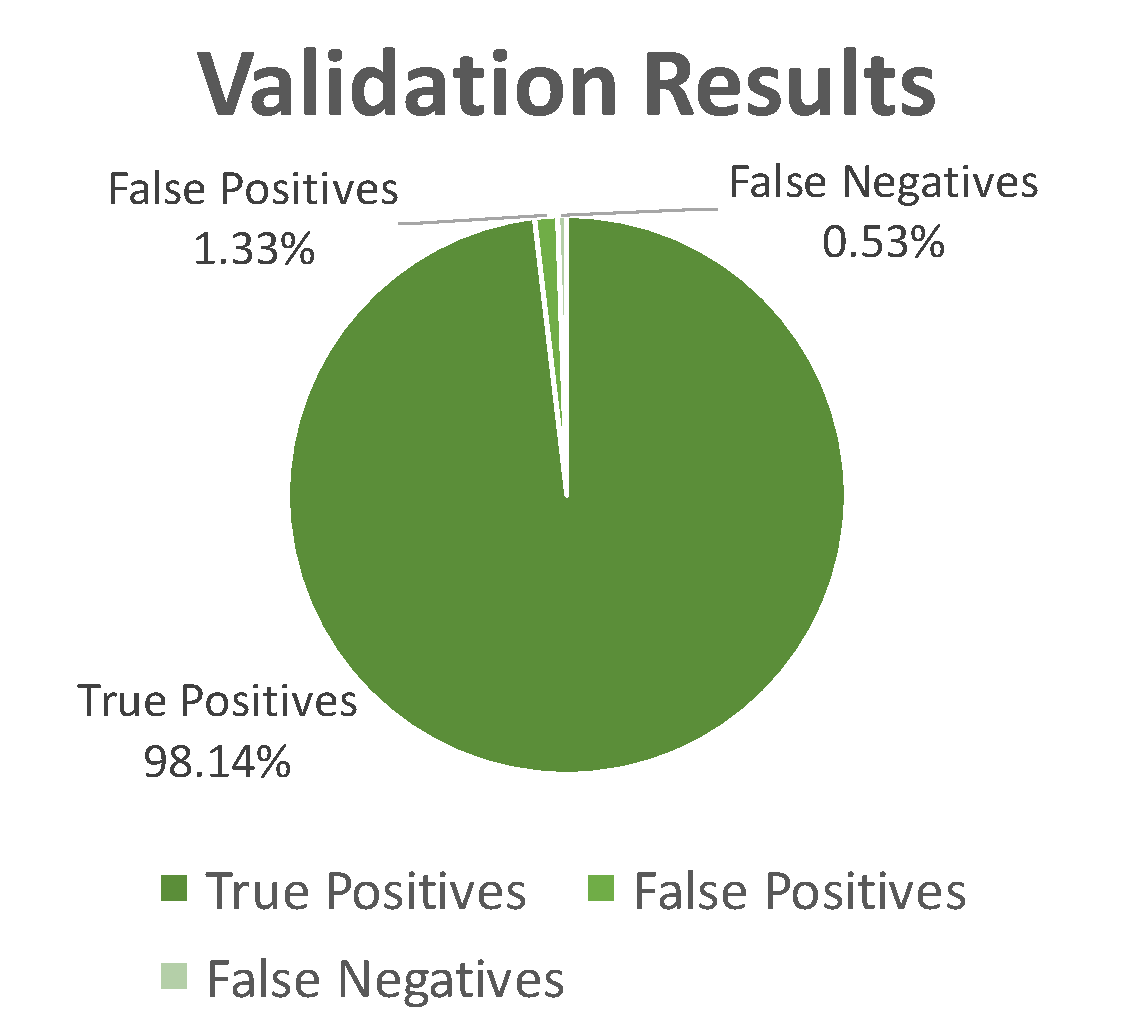
\includegraphics[width=0.5\linewidth]{img/validation_results}
            \caption{Pie chart showing the manual validation results including true positives, false positives, and false negatives.}
            \label{fig:validation_results}
        \end{figure}
    
    
%----------------------------------------
% QUALITY ANALYSIS RESULTS
%----------------------------------------
\section{Quality Analysis}


	%----------
    % APPROACH
    %----------
    \subsection{Approach}
    
    	The results of the application have provided many possibilities for statistical analysis since numerous statistics can be calculated from the generated approach data.  This can be seen in \Cref{subfig:stableness_results,subfig:unstable_landing_results,subfig:unstable_parameters,subfig:landing_type_results} in which a sample of the possible results were calculated from the experiments of the 100 flights used in this research.  With these various results, trends can be found in the data that has been analyzed.  For example, we can see in \Cref{subfig:stableness_results} that out of the 377 approaches in the sample data, 74.27\% (280) were stable and 25.73\% (97) were unstable.  By drilling down into that data, we can see the frequency for each of the landing types for stable and unstable approaches.  Figure~\ref{subfig:landing_type_results} depicts this more detailed information and shows that full-stop landings occur most frequently for both stable and unstable approaches.  This result is not very surprising for stable approaches; however, it is very undesirable for unstable approaches.  If we look even further into the proportions for unstable approaches alone (\Cref{subfig:unstable_landing_results}), we see that an unstable approach resulted in a go-around only 20.62\% of the time.  This is far lower than the hopeful 100\%, but was expected to be approximately 20\% by our aviation safety experts.  As mentioned previously, this is largely due to pilot misjudgment since all the analyzed flights were piloted by aviation students; meaning they are still learning and are not yet professionals.
    
    When looking at the unstable approaches and the parameters that caused them (\Cref{subfig:unstable_parameters}), additional interesting results can be found.  We found the parameter that was exceeded the most was heading with 52 occurrences.  Heading was not predicted to be the leading cause of unstable approaches, but our safety experts believe the 10$^\circ$ threshold (as defined in \Cref{tab:approach_thresholds}) may be too strict.  Indicated airspeed was the second highest, but was predicted to be the leading cause since it was stated by our aviation safety experts to be a trend for UND's student pilots to be going too fast on final approaches.
    
    \begin{figure}
    	\centering
        \subfloat[Pie chart showing the number of stable approaches compared to the number of unstable approaches.\label{subfig:stableness_results}]{
        	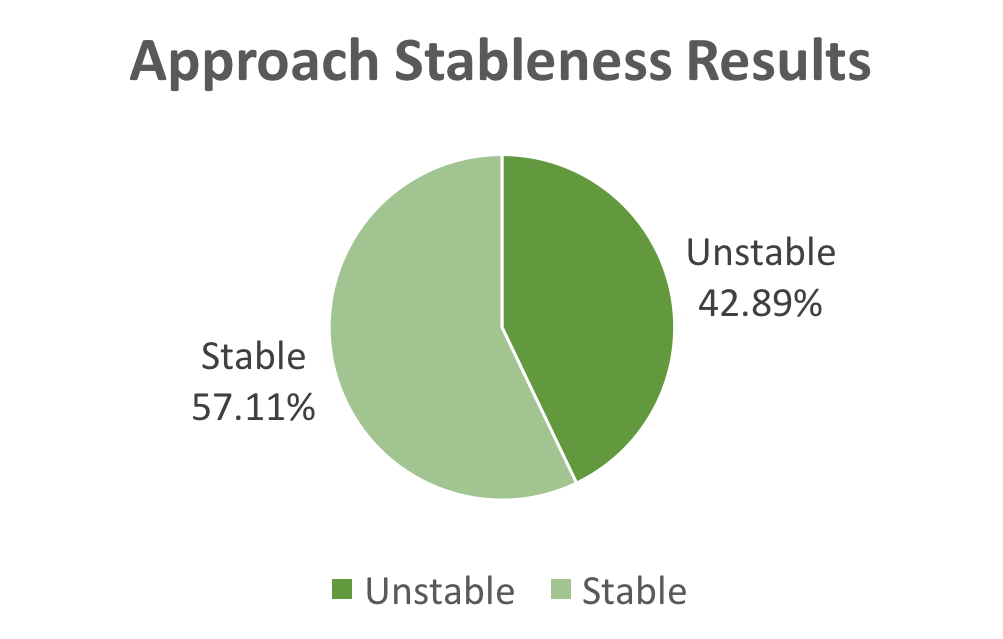
\includegraphics[width=0.45\linewidth]{img/stableness_results}
        }\hfill%
        \subfloat[Frequency of the occurrences of each landing type for stable and unstable approaches.\label{subfig:landing_type_results}]{
        	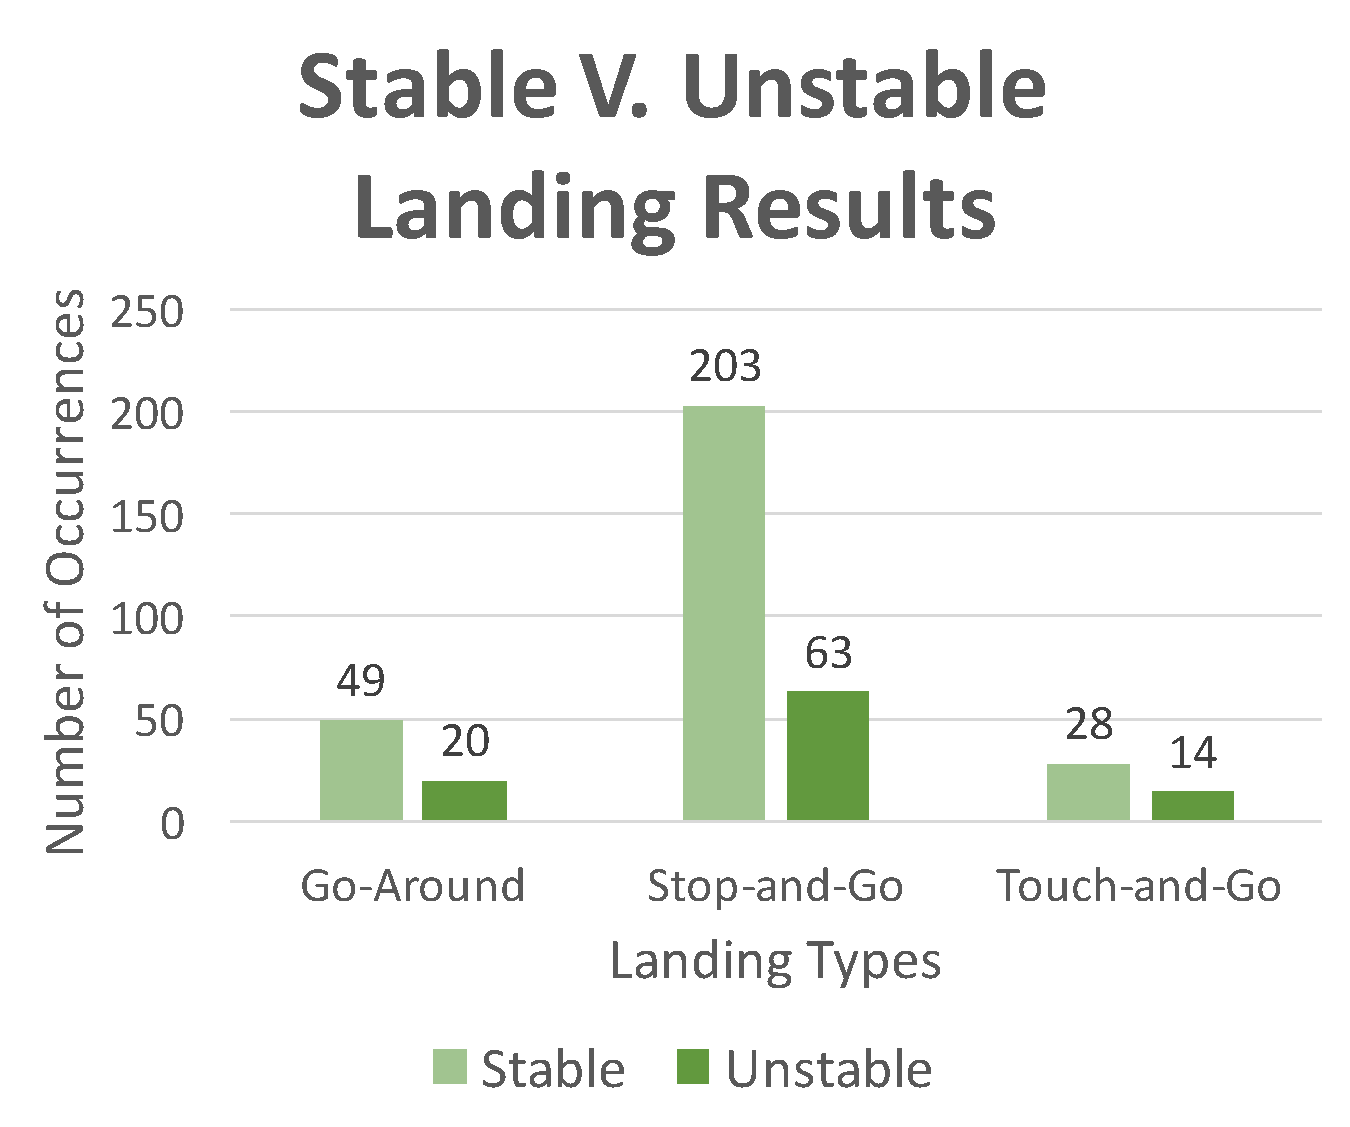
\includegraphics[width=0.45\linewidth]{img/landing_type_results}
        }%
        
        \subfloat[Pie chart comparing the number of occurrences for each landing type after an unstable approach.\label{subfig:unstable_landing_results}]{
        	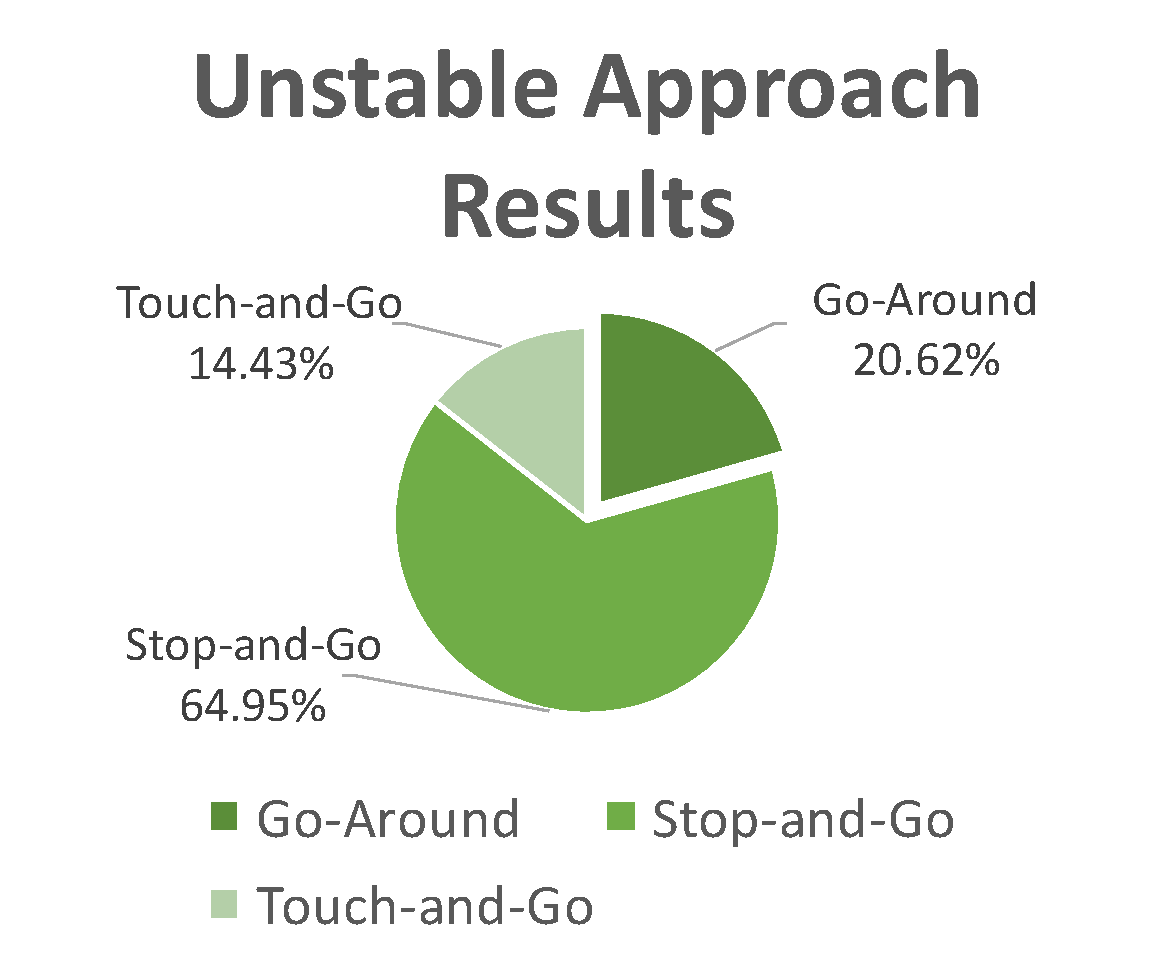
\includegraphics[width=0.45\linewidth]{img/unstable_approach_landing_results}
        }\hfill%
        \subfloat[Frequency of parameters that caused an aircraft to be unstable during an approach.  Note that a single approach can have multiple unstable parameters, which causes the sum of the occurrences to not equal the total number of unstable approaches.\label{subfig:unstable_parameters}]{
        	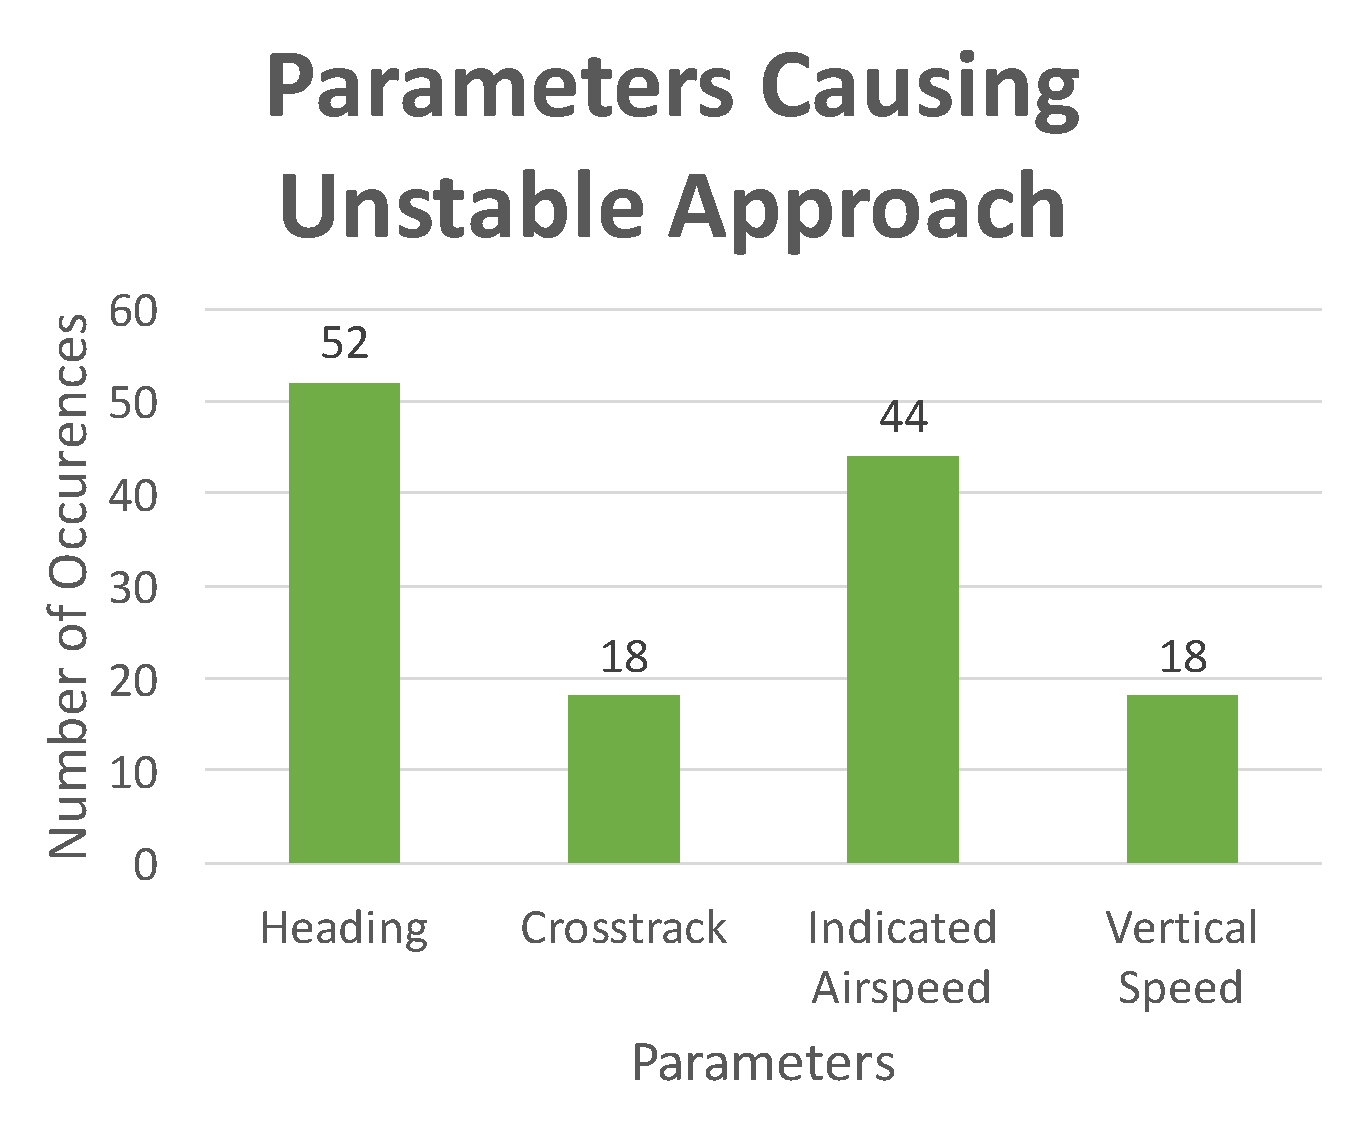
\includegraphics[width=0.45\linewidth]{img/unstable_parameter_results}
        }%
        \caption{Sample set of the statistics and trends that can be found from the automated analysis results.}
        \label{fig:example_statistics}
    \end{figure}
    
    
    Another interesting set of statistics that can be drawn from the analysis are parameter value frequencies.  Creating histograms of the values for each parameter during all Approach phases can show the values that occur most frequently (highest density).  \Cref{subfig:approach_ias_hist,subfig:approach_vsi_hist,subfig:approach_cross_track_hist,subfig:approach_heading_hist} visualize these histograms and give the corresponding mean and standard deviation values.  These graphs are able to show how well pilots are adhering to the published stabilized approach criteria (see \Cref{tab:approach_thresholds}).  As mentioned previously, the standard deviations will be used in defining the grading metrics and will be discussed in more detail later in this Chapter.
    
    \begin{figure}
    	\centering
        \subfloat[Indicated airspeed ($\mu = 64.401, \sigma = 4.535$)\label{subfig:approach_ias_hist}]{
        	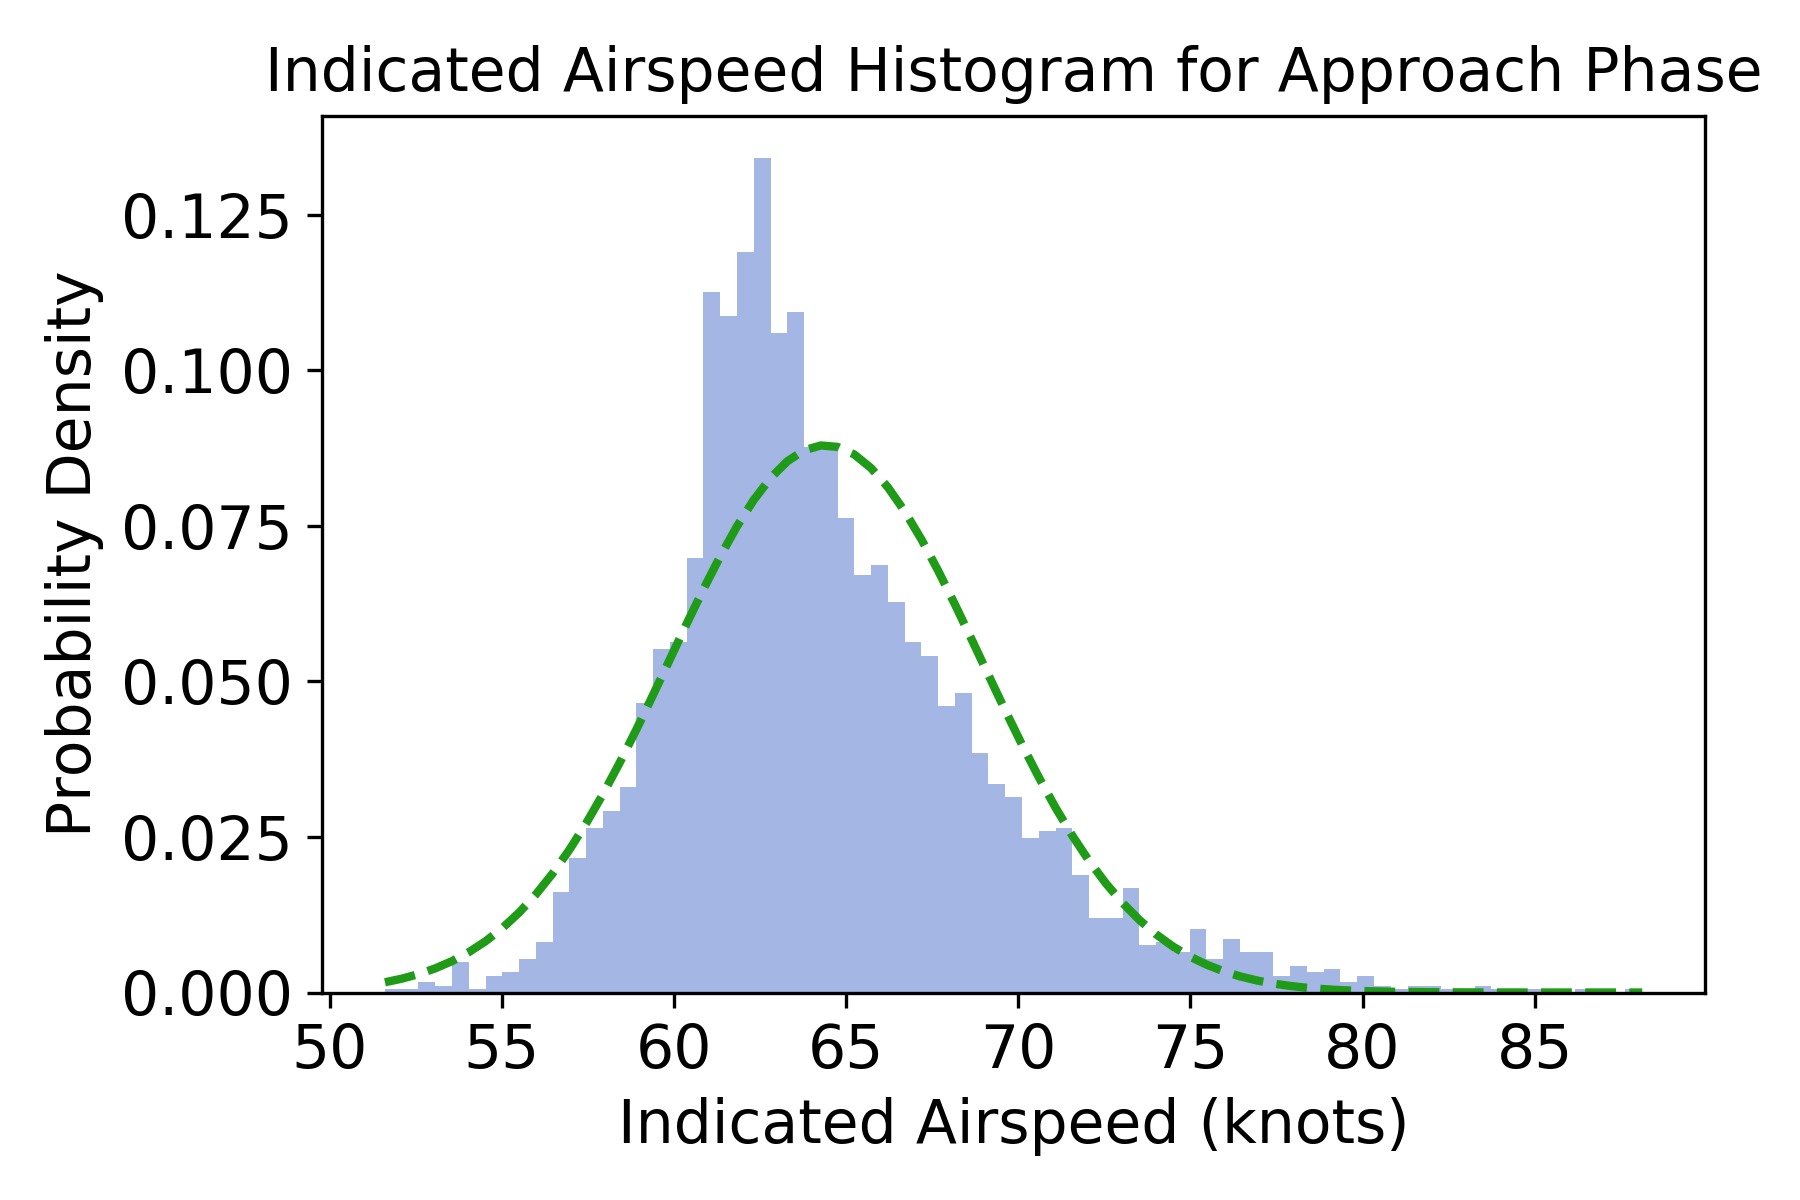
\includegraphics[width=0.45\linewidth]{img/ias_hist}
        }\hfill%
        \subfloat[Vertical speed indicated ($\mu = -364.528, \sigma =181.210$) \label{subfig:approach_vsi_hist}]{
        	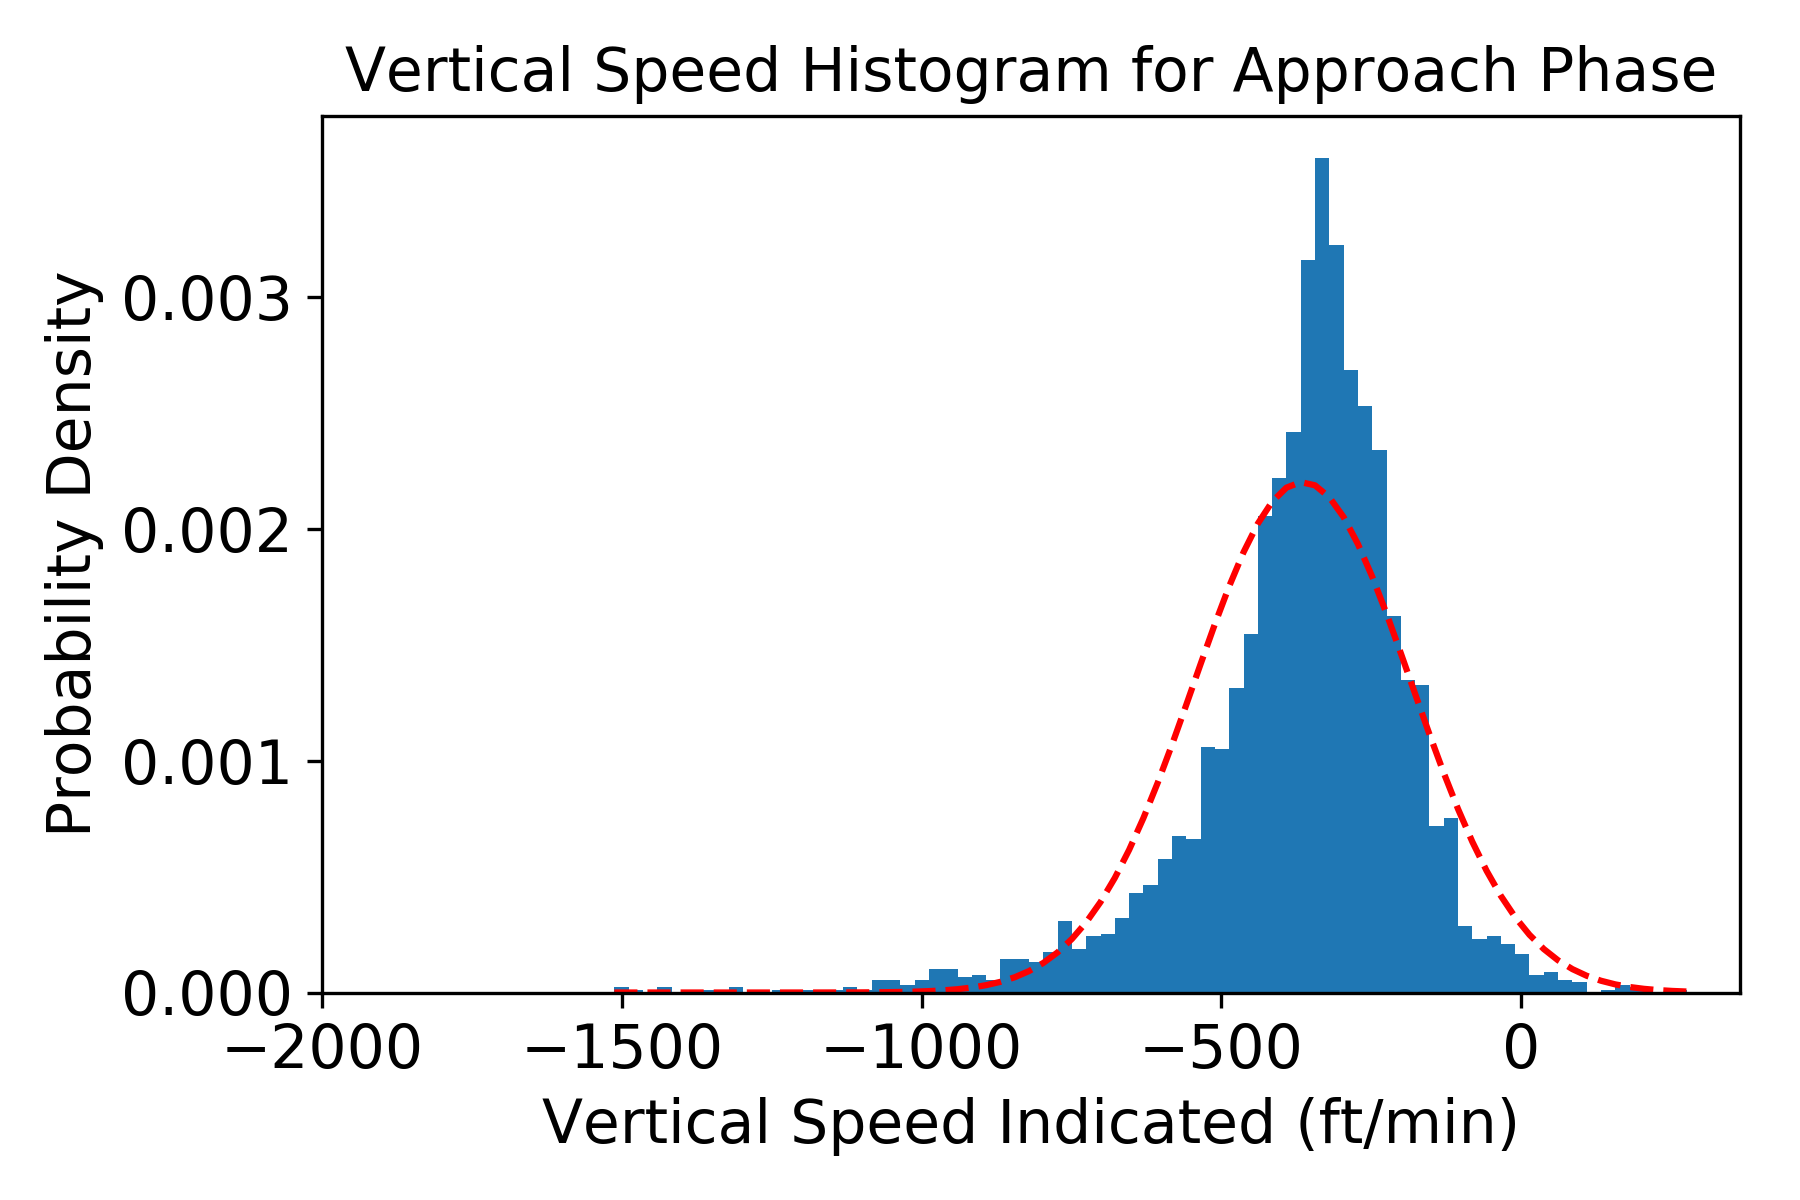
\includegraphics[width=0.45\linewidth]{img/vsi_hist}
        }%
        
        \subfloat[Cross track error ($\mu = -4.542, \sigma = 15.499$) \label{subfig:approach_cross_track_hist}]{
        	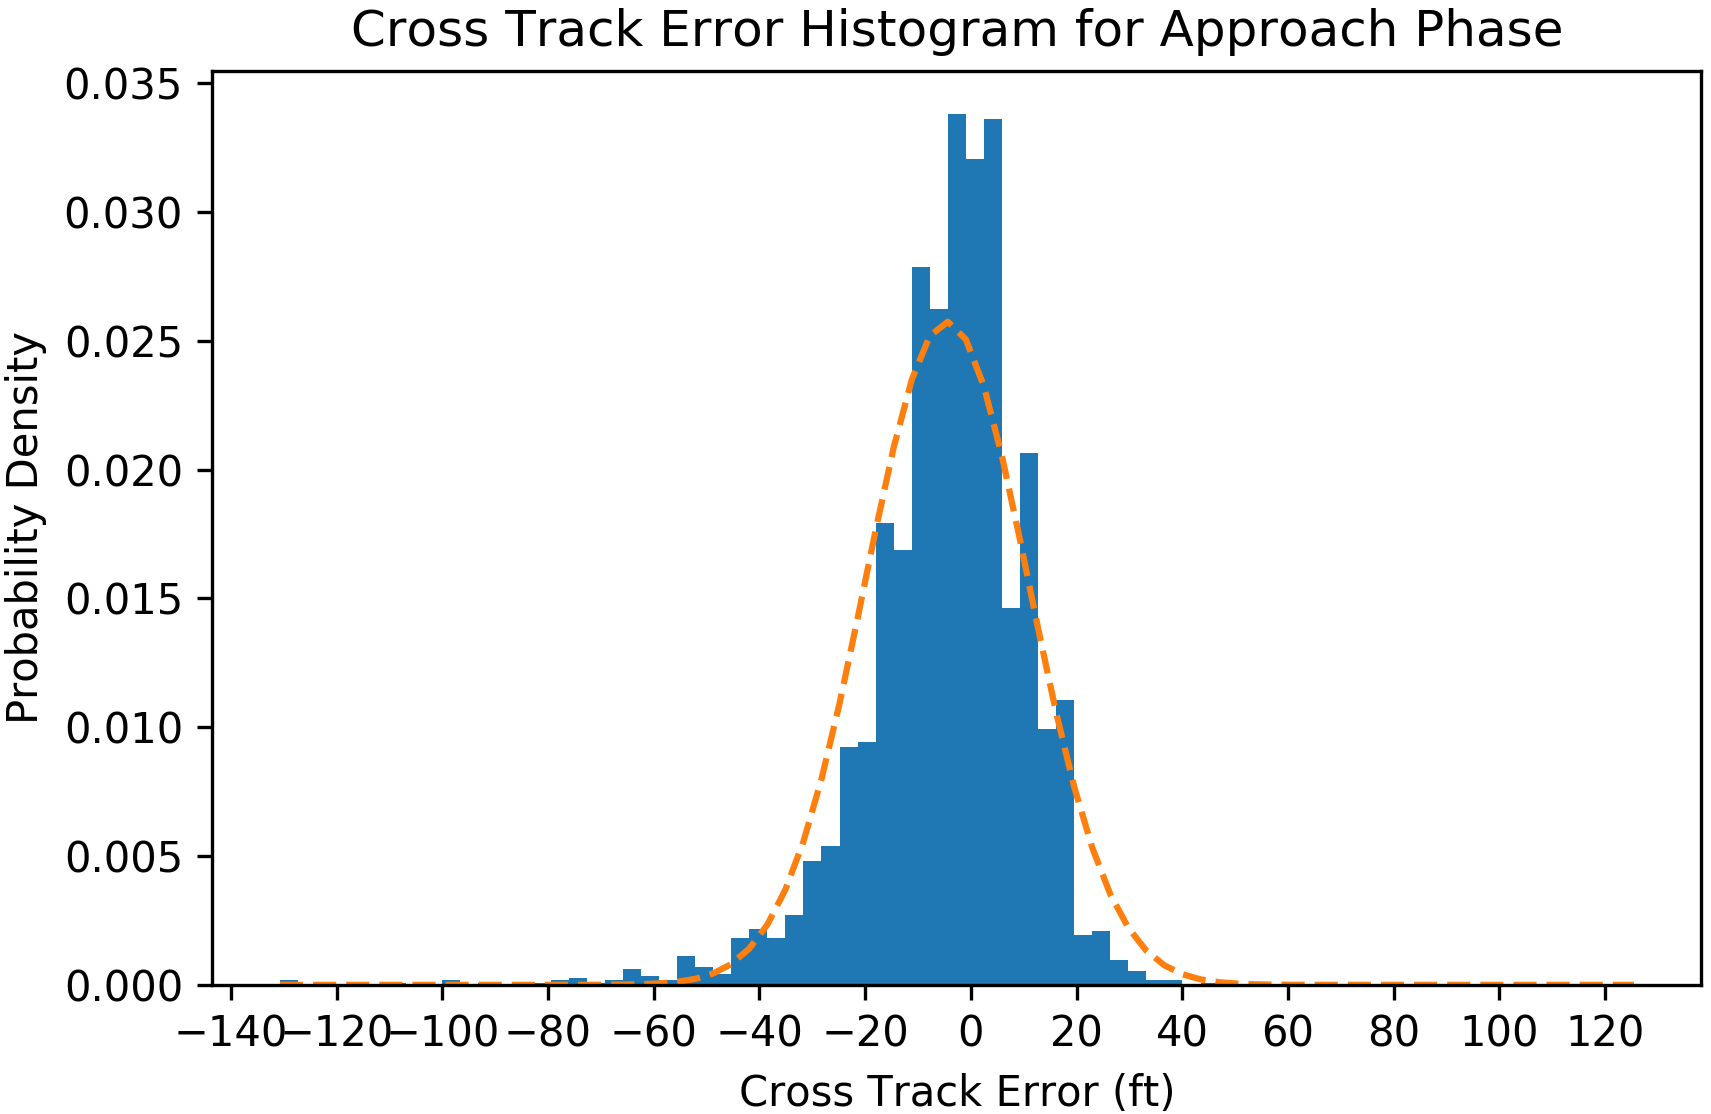
\includegraphics[width=0.45\linewidth]{img/cross_track_hist}
        }\hfill%
        \subfloat[Heading error ($\mu = 1.958, \sigma = 4.761$) \label{subfig:approach_heading_hist}]{
        	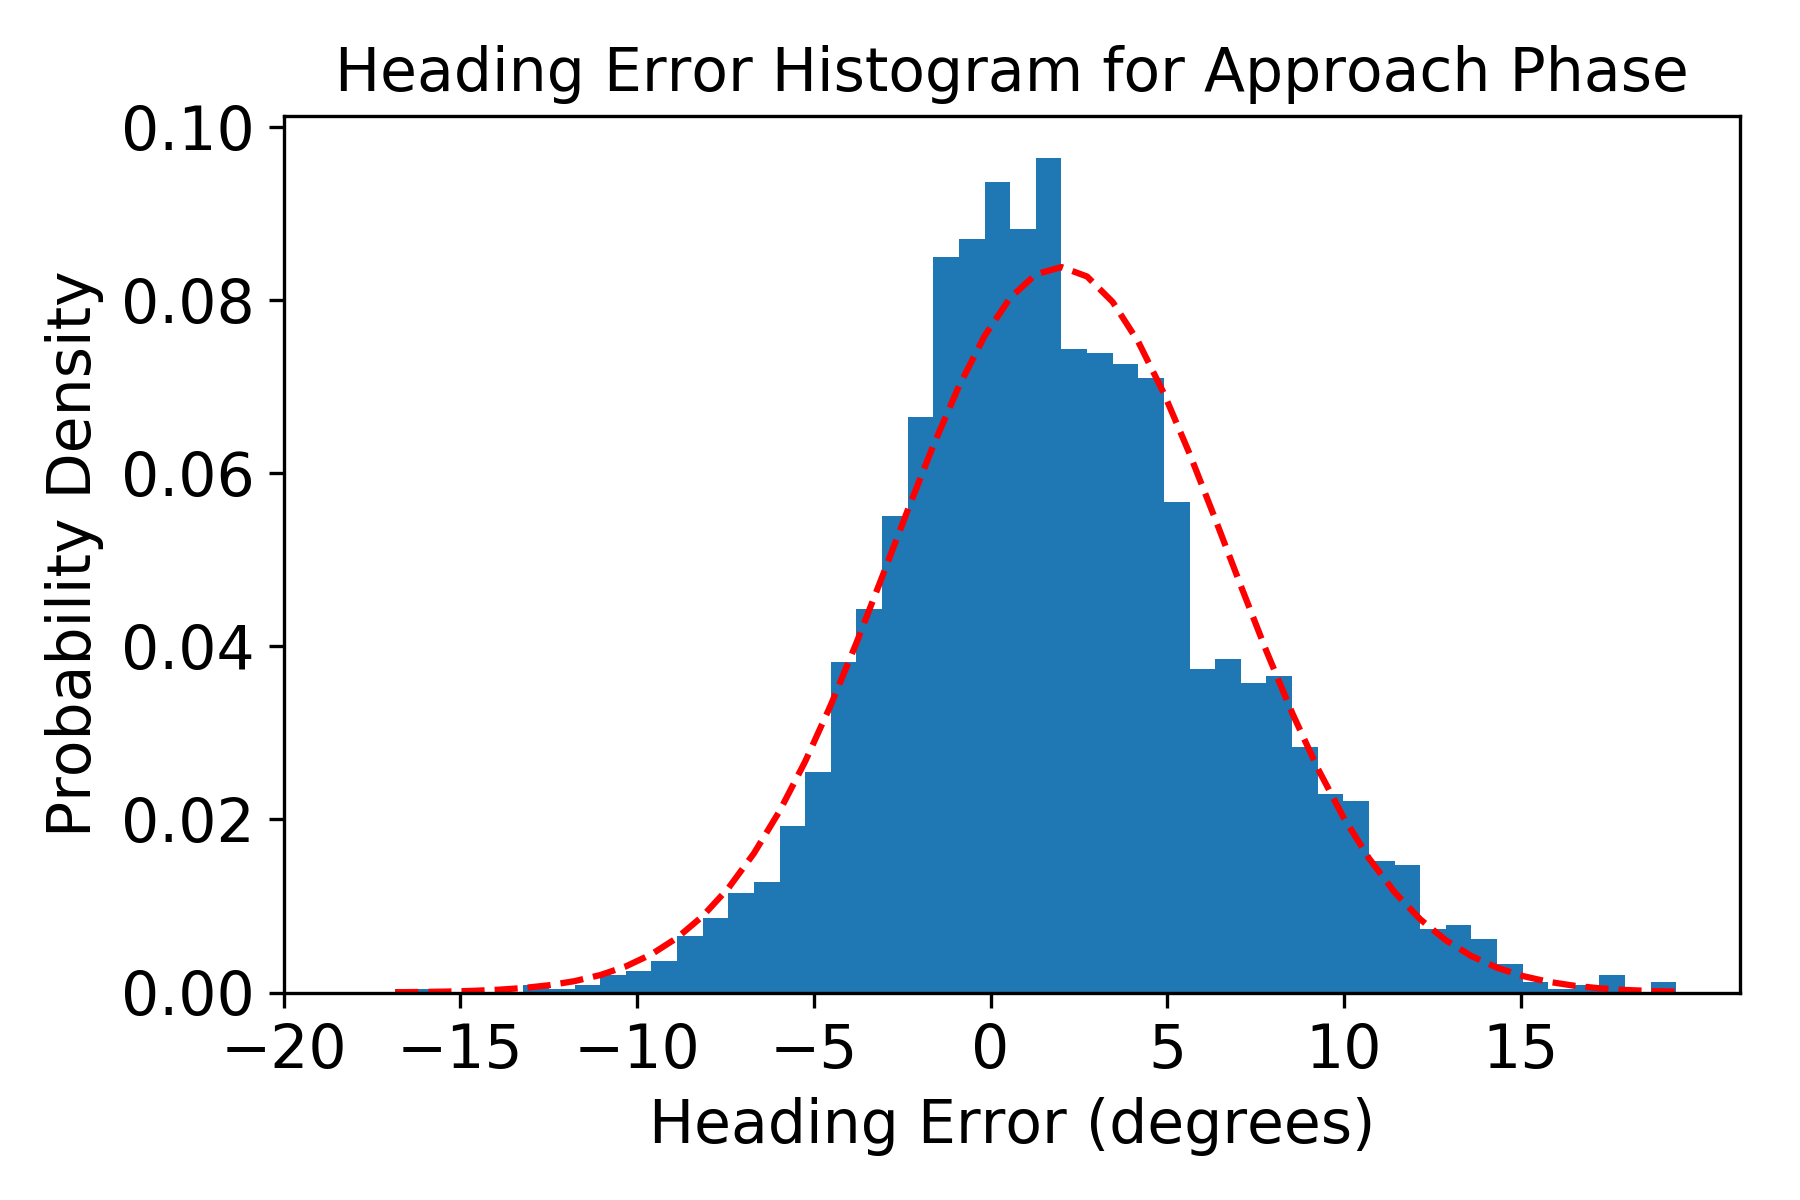
\includegraphics[width=0.45\linewidth]{img/heading_hist}
        }%
        \caption{Histograms showing the frequencies of values for each parameter during all Approach phases.  Each graph also has a dotted best-fit line to show how close the frequencies adhere to a normal distribution.}
        \label{fig:approach_histograms}
    \end{figure}
    
    
    	%----------
        % FINAL TURN
        %----------
        \subsubsection{Final Turn.}
        
        	\note{Insert charts showing the number of small/large under/overshoots.}
            
        
        %----------
        % APPROACH
        %----------
        \subsubsection{Self-defined glide path.}
        
        	\note{Not sure.  May remove this section since the Web Interface shows exactly the charts that can be created.}


%----------------------------------------
% GRADING METRICS: DEFINE FROM PARAMETER FREQUENCIES
%----------------------------------------
\section{Grading Metrics:  Define From Parameter Frequencies}

	%----------
    % APPROACH
    %----------
    \subsection{Approach}
    
    	
        %----------
        % IAS
        %----------
    	\subsubsection{Indicated airspeed between 55 and 75 knots.}
        
            
        
        
        %----------
        % VSI
        %----------
    	\subsubsection{Vertical speed indicated greater than -1000 ft/min.}
        
            
        
        
        %----------
        % CROSS TRACK ERROR
        %----------
    	\subsubsection{Absolute cross track error less than 50 ft.}
        
            
            
            
        %----------
        % HEADING ERROR
        %----------
    	\subsubsection{Absolute heading error less than 10 degrees.}
        
            

%----------------------------------------
% GRADING METRICS: RESULTS
%----------------------------------------
\section{Grading Metrics:  Experiment Results}

	\note{Results found from using metrics on analysis results.}
    
    
%----------------------------------------
% WEB INTERFACE
%----------------------------------------
\section{Web Interface}

	This Section details the newly developed web pages for the NGAFID, which dynamically display results based on the user's chosen filters.  At the time of this writing, there have been new tools developed for the Approach, Final Turn, and self-defined glide path analyses.  Each tool will be discussed further in the subsequent Subsections.
    
    
    %----------
    % APPROACH
    %----------
    \subsection{Approach}
    
    	A new web page was implemented in the NGAFID for the purpose of dynamically displaying the Approach analysis results produced by the \toolname\ to users (\Cref{fig:approach_tool_screenshot}).  The results are given in four tabs, one for each parameter, as histograms over a specified date range.  A user is able to dynamically add additional date ranges, which will create an additional series in the chart for comparison.  This feature can be used to detect changes in trends over time.  A user is also, optionally, able to filter the results to an airport and further filter to a single runway.  This will allow users to identify trends that are potentially occurring at a specific runway but not at any other runways.
    
    	\begin{figure}
    		\centering
            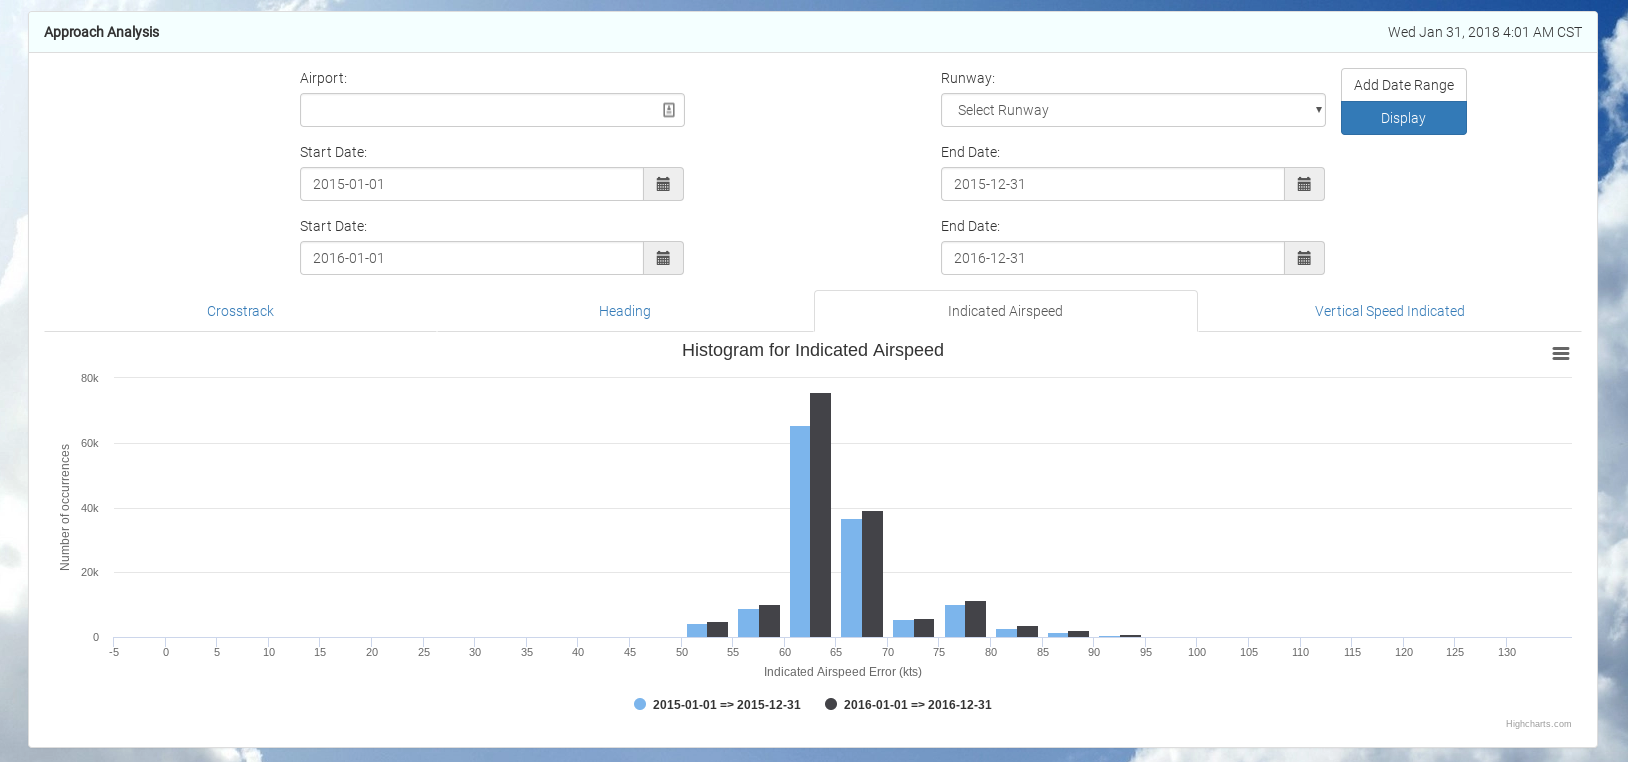
\includegraphics[width=\linewidth]{img/approach_tool_screenshot}
            \caption{A screenshot of the Approach analysis tool on the NGAFID.  It is showing the histogram for indicated airspeed error with two date range filters: 2015-01-01 to 2015-12-31 and 2016-01-01 to 2016-12-31.  The frequency of exceedances can be seen with all values that fall outside of the 55-75 knots range.}
            \label{fig:approach_tool_screenshot}
    	\end{figure}
    
    
    %----------
    % FINAL TURN
    %----------
    \subsection{Final Turn}
    
    	The tool developed for analyzing Final Turn phases in the NGAFID was implemented with two modes:  \textit{(i)} ``Single Flight'' and \textit{(ii)} ``Aggregate''.
    
    	For the ``Single Flight'' mode, the user can input an ID for a specific flight they'd like to analyze (\Cref{fig:single_ttf_screenshot}).  Once the user clicks the ``Display Single Flight'' button, the interactive map then dynamically transitions to the first approach for that flight.  The map will only display one approach at a time; although, there are tabs across the top for each approach which the user can choose.  Once a different tab is chosen, the map automatically transitions the view to that corresponding approach.  The flight path shows different color codings for the separate Final Turn, Approach, and Landing phases as well as different colors for the Final Turn specifically depending on the severity of the turn error.  A Level 1 turn error will be colored yellow, while a Level 2 turn error will be colored red.  If the turn error is less than the Level 1 criteria, it is colored green.  The user is also able to download a PNG screenshot of the map by clicking the ``Download PNG'' button.
        
        For the ``Aggregate'' mode; the user can choose a specific airport, runway, and month and year combination; which will then display all the approaches that occurred at the chosen runway during the chosen time-frame (\Cref{fig:agg_ttf_screenshot}).  This mode allows a user to see trends in Final Turn phases during a given time span.  This mode displays the same color code scheme as the ``Single Flight'' mode.
    
    	\begin{figure}
    		\centering
            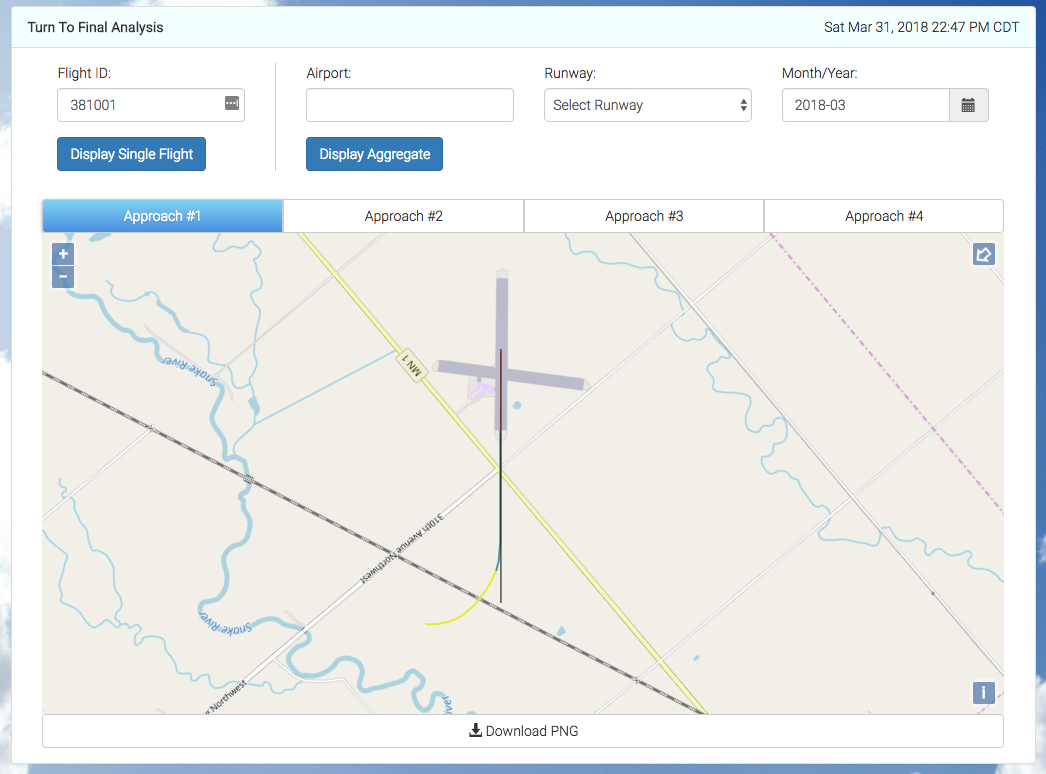
\includegraphics[width=\linewidth]{img/single_ttf_screenshot}
            \caption{A screenshot of the Final Turn analysis tool on the NGAFID in ``Single Flight'' mode.  It is currently showing Approach \#1 for Flight ID \#381001.  Approach \#1 shown here had a Level 1 (yellow color code) undershoot.}
            \label{fig:single_ttf_screenshot}
    	\end{figure}
        
        \begin{figure}
    		\centering
            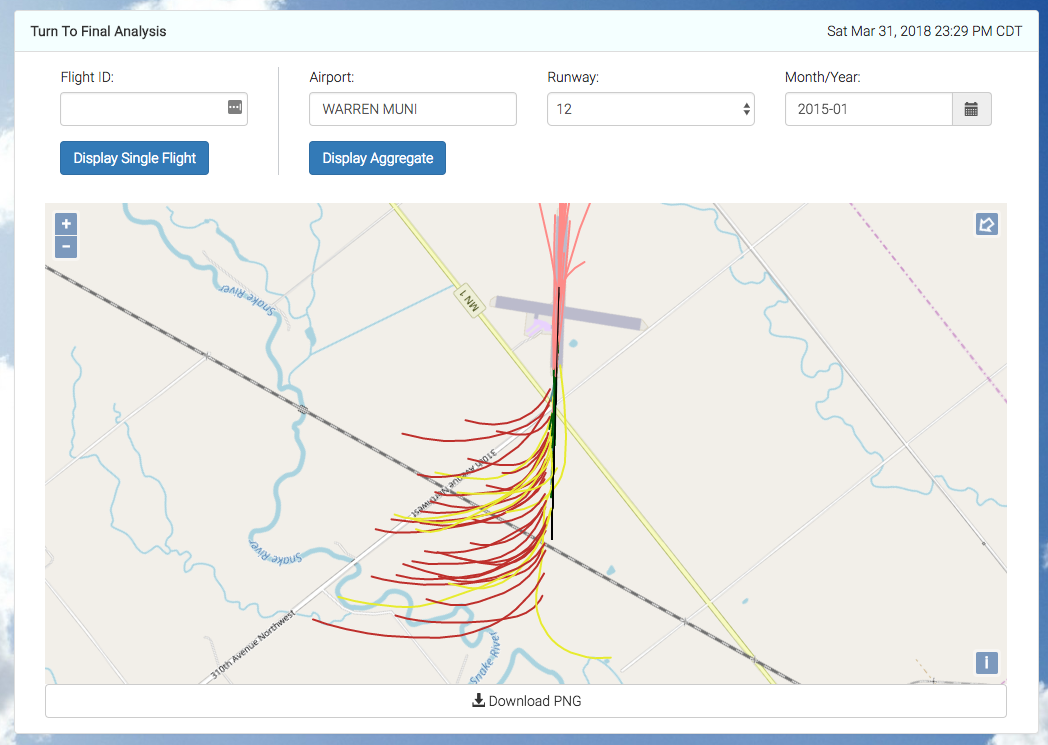
\includegraphics[width=\linewidth]{img/agg_ttf_screenshot}
            \caption{A screenshot of the Final Turn analysis tool on the NGAFID in ``Aggregate'' mode.  It is currently showing all approaches at the Warren Municipal Airport (KD37) for Runway 12 during the month of January 2015.  The many red and yellow lines coming in from the left side mean that a majority of the turns were Level 1 \& 2 undershoots.}
            \label{fig:agg_ttf_screenshot}
    	\end{figure}
    
    %----------
    % SELF-DEFINED
    %----------
    \subsection{Self-Defined Glide Path}
    
    	The tool implemented in the NGAFID for displaying the results of the self-defined glide path analysis currently only supports an aggregate mode (\Cref{fig:self_defined_screenshot}).  It works similarly to the Final Turn tool as the user chooses an airport, runway, and month and year combination.  This will then display a sideways histogram of all the approaches at the given runway during the given time-frame.  The y-axis shows glide path angles from $0^\circ$ to $10^\circ$ in $5^\circ$ increments, and the x-axis shows the number of occurrences that fell within each angle bin.  Lastly, the user can download an image of the displayed chart by clicking the ``hamburger'' menu button.
    
    	\begin{figure}
    		\centering
            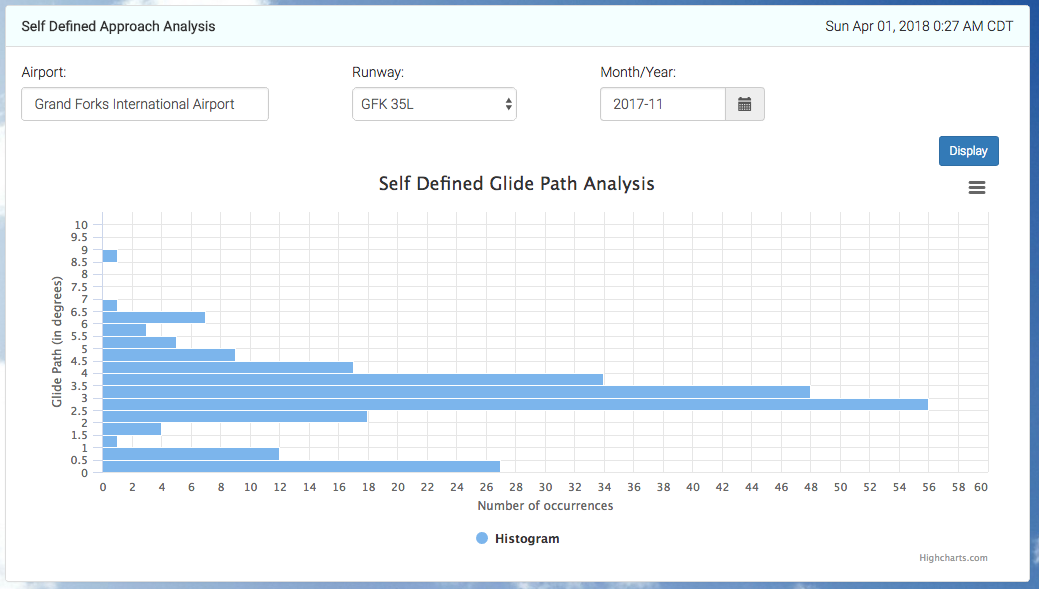
\includegraphics[width=\linewidth]{img/self_defined_screenshot}
            \caption{A screenshot of the Self-Defined Approach analysis tool on the NGAFID.  It is currently showing all approaches at the Grand Forks International Airport (KGFK) for Runway 35L during the month of November 2017.  It displays a sideways histogram with glide path angles on the y-axis and the number of occurrences for each angle on the x-axis.}
            \label{fig:self_defined_screenshot}
    	\end{figure}


%----------------------------------------
% PERFORMANCE
%----------------------------------------
\section{Performance}

	A secondary aspect of this research is to minimize the execution time so  the analysis only adds a minimal amount of time to a flight being imported into the NGAFID system.  The results of the benchmarking tests showed that the linearly executing application ran for an average of XXX.XXX seconds over the 100 randomly tested flights.  On the other hand, the parallel application ran for an average of XX.XXX seconds over the same flights.  This means the average per-flight execution times for the linear and parallel applications were X.XXX and X.XXX seconds, respectively.  As a result, the parallelized application had a XX.XXX\% speedup, which is fairly significant.  %A summary of the benchmarking tests and other relevant statistics are given in \Cref{tab:performance_results}.
    \note{Fill in timing results.}
    
    As further evidence, the parallel application was tested on a larger subset of flights to see if the average execution time remained stable, in which it was tested on 5,272 flights.  For this test, the parallel application was able to analyze the data and insert all the results into the database in XXXX.XXX seconds.  This gives a per-flight execution time of X.XXX seconds, which is slightly less than the average for 100 flights.  The reasoning behind this can most likely be attributed to the fact that spinning up the sub-processes creates a substantial overhead.  Thus, the longer the application is able to execute, the greater performance gain will be received.  This will, of course, start to show diminishing returns as with any other parallel computing application.
    
    
    \begin{table}[tb]
        \caption{\small{Performance of Linear v. Parallel Execution Times}}
        \vspace{3pt}
        \label{tab:performance_results}
        \centering
        \begin{tabular}{@{} >{\centering\arraybackslash} m{.23\linewidth} S[table-format=3.3] S[table-format=2.3] @{}}
            \hline\noalign{\smallskip}
            \bfseries Run & \bfseries Linear (sec) & \bfseries Parallel (sec) \\
            \noalign{\smallskip}
            \hline
            \noalign{\smallskip}
             1 & 591.935 & 57.295 \\ \hline
             2 & 576.774 & 60.282 \\ \hline
             3 & 586.009 & 57.830 \\ \hline
             4 & 597.643 & 62.489 \\ \hline
             5 & 591.170 & 57.578 \\ \hline
             6 & 585.834 & 62.702 \\ \hline
             7 & 593.711 & 65.064 \\ \hline
             8 & 587.177 & 66.167 \\ \hline
             9 & 586.059 & 58.108 \\ \hline
            10 & 590.012 & 56.501 \\ \hline
            \hline
            \bfseries Average           & 588.632 & 60.402   \\ \hline
            \bfseries Latency / flight  &   5.886 &  0.604   \\ \hline
            \bfseries Speedup           &         & 90.255\% \\ \hline
        \end{tabular}
    \end{table}
    
    
    
    